\section{Lattice Theory}\label{lattice}
The static analysis we want to perform utilises the mathematical theory of lattices together with a monotone function to guarantee that the analysis will terminate.
This theory will be described in the following.

\paragraph{Partial orders}
A lattice is a specialisation of a partial order which will be described in the following.
A partial order is a mathematical structure $L = (S, \sqsubseteq)$ where S is a set and $\sqsubseteq$ is a binary relation where the following conditions are satisfied:
\begin{itemize}
  \item Reflexivity: $\forall x \in S : x \sqsubseteq$
  \item Transitivity: $\forall x,y,z \in S : x \sqsubseteq y \wedge y \sqsubseteq z \Rightarrow x \sqsubseteq z$
  \item Antisymmetry: $\forall x,y \in S: x \sqsubseteq y \wedge y \sqsubseteq x \Rightarrow x = y$
\end{itemize}

\todo{maybe something about what this means and implications?}

\paragraph{Least upper bound}
As the name states, a least upper bound is the least of all upper bounds.
An upper bound y of a set X where $ X \subseteq S$ and S is a partial order is written as $X \sqsubseteq y$.
y is an upper bound of X if we have that $\forall x \in X : x \sqsubseteq y$.

We can now define the least upper bound, written as $\sqcup X$:
\[X \sqsubseteq \sqcup X \wedge \forall y \in S : X \sqsubseteq y \Rightarrow \sqcup X \sqsubseteq y\]

The greatest lower bound $\sqcap X$ can be defined by the same logic.

\paragraph{Lattice}
A lattice can now be defined as a partial order in which $\sqcup X$ and $\sqcap X$ is defined for all $X \subset S$.
It should be noted  that a lattice must have a unique largest element $\top$ defined as $\top = \sqcup S$ and unique smallest element $\bot$ 

\begin{figure}
\begin{center}
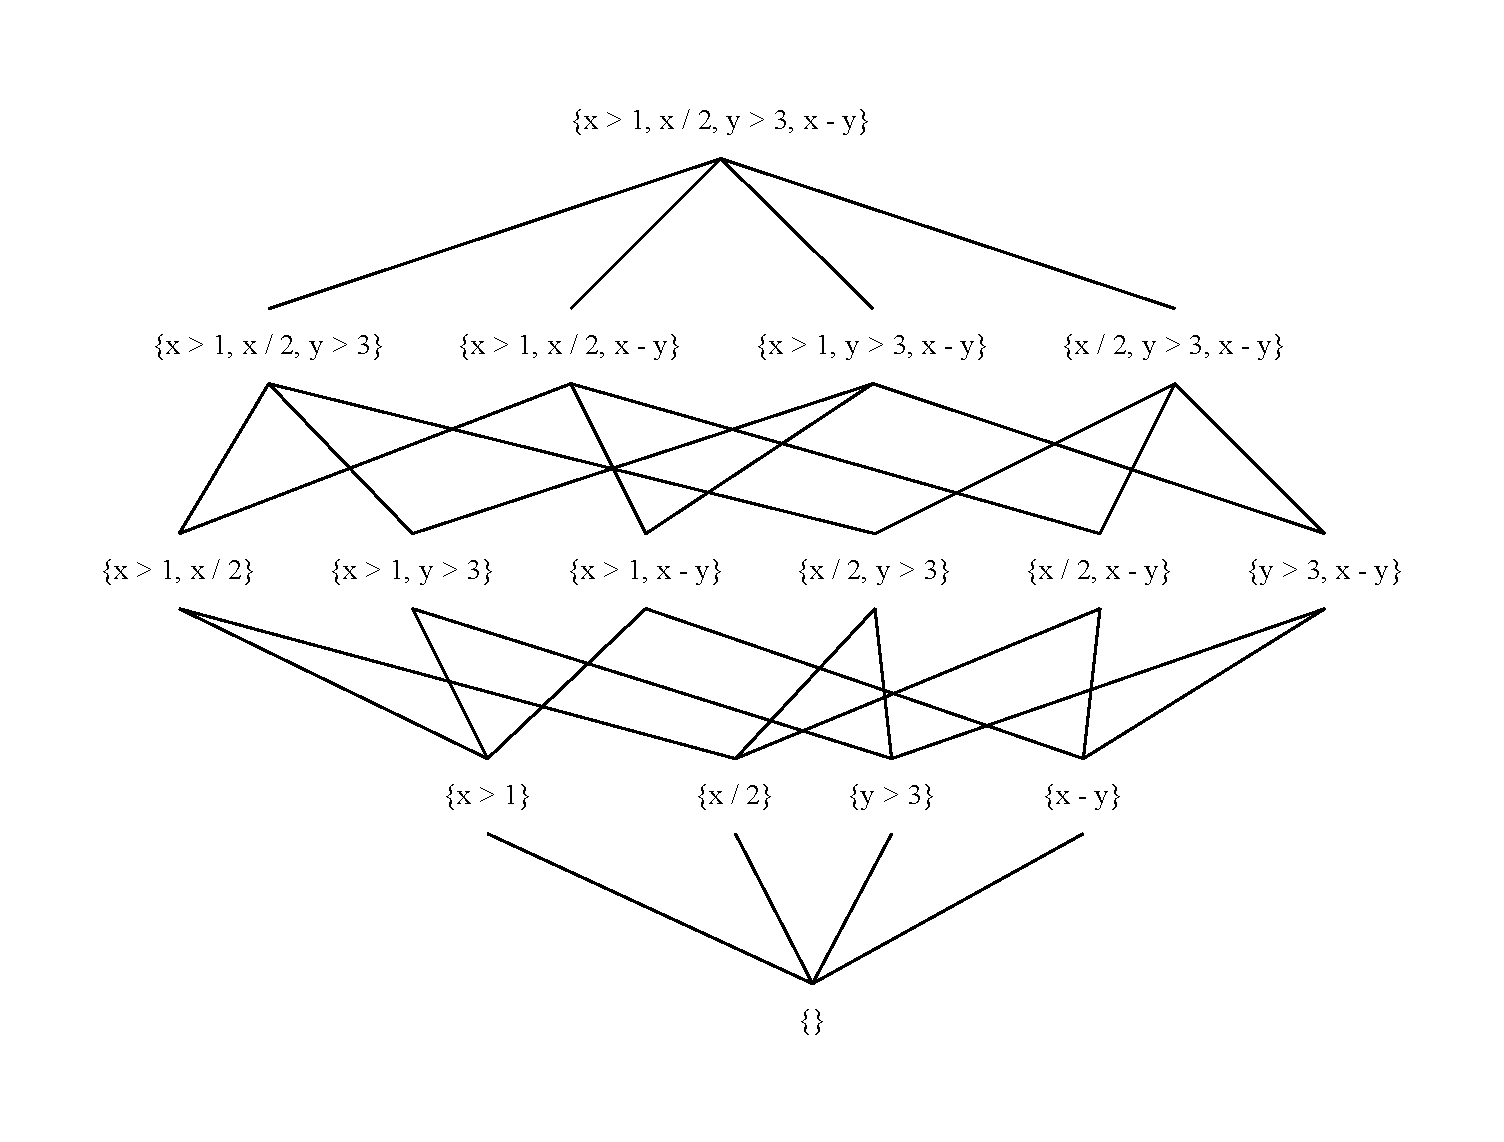
\includegraphics[width=\textwidth]{figures/dot_files/lattice_example.pdf}
\end{center}
\caption{A lattice with four expressions.}
\label{lattice_example}
\end{figure}

In \cref{lattice_example} a lattice with four elements is depicted.
These four elements are deduced from a subset of the general example program on \cref{theory:general_code_example}(in order to keep the size of the lattice manageable).
The subset can be seen on \cref{theory:general_code_example_small}.

\begin{lstlisting}[style=python, caption={The general code example used throughout the theory chapter}, label={theory:general_code_example_small}]
  x = input()
  x = int(x)
  while x > 1:
      y = x / 2
      if y > 3:
          x = x-y
  print(x)
\end{lstlisting}

This lattice is defined by the set of four expressions $\{x > 1, x / 2, y > 3, x - y \}$.
In general the set $A$ defines a lattice $(2^A, \sqsubseteq )$ where $\top = \emptyset$, $\bot = A$, $x\sqcup y = x \cup y$ and $x \sqcap y = x \cap y$.

Every analysis requires the lattice to contain certain elements of the program in order to work.
Examples range from expressions or assignments to variables.
The presented type of lattice is used in analyses that depend on information about the expressions in a program.
One example of such analysis is 'available expressions' which is presented in \citet[p.~22]{schwartzbach}.
This analysis finds expressions that are \emph{available} at a program point.
An available expression is an expression that has already been calculated earlier in the execution.
Finding available expressions can be used to optimize the program by saving the calculation and thus avoid recalculating it.



